\documentclass[a4paper,10pt]{article}
\usepackage[utf8]{inputenc}
\usepackage[spanish]{babel}
\usepackage[affil-it]{authblk}
\usepackage{enumerate}
\usepackage{graphicx}
\usepackage{hyperref}
\usepackage{amsmath}
\usepackage{amssymb}
\usepackage{cancel}
\usepackage{tikz}
\usetikzlibrary{calc}
\usepackage{listings}
\usepackage{subfig}
\usepackage{float}

%Boxes
\newcommand*{\boxcolor}{blue}
\makeatletter
\renewcommand{\boxed}[1]{\textcolor{\boxcolor}{%
\tikz[baseline={([yshift=-1ex]current bounding box.center)}] \node [rectangle, minimum width=1ex,rounded corners,draw] {\normalcolor\m@th$\displaystyle#1$};}}
 \makeatother

%Constants
\newcommand{\euler}{\mathrm{e}}
\newcommand{\im}{\mathrm{i}}

\title{Mecánica Clásica Tarea \# 2}
\author{Favio Vázquez\thanks{Correo: favio.vazquezp@gmail.com}}\affil{Instituto de Física. Universidad Nacional Autónoma de México}
\date{}

\begin{document}

\makeatletter
\def\@maketitle{%
  \newpage
  \null
  \vskip 2em%
  \begin{center}%
  \let \footnote \thanks
    {\Large\bfseries \@title \par}%
    \vskip 1.5em%
    {\normalsize
      \lineskip .5em%
      \begin{tabular}[t]{c}%
        \@author
      \end{tabular}\par}%
    \vskip 1em%
    {\normalsize \@date}%
  \end{center}%
  \par
  \vskip 1.5em}
\makeatother

\maketitle

%Styling for code
\definecolor{codegreen}{rgb}{0,0.6,0}
\definecolor{codegray}{rgb}{0.5,0.5,0.5}
\definecolor{codepurple}{rgb}{0.58,0,0.82}
\definecolor{backcolour}{rgb}{0.95,0.95,0.92}
 
\lstdefinestyle{mystyle}{
    backgroundcolor=\color{backcolour},   
    commentstyle=\color{codegreen},
    keywordstyle=\color{magenta},
    numberstyle=\tiny\color{codegray},
    stringstyle=\color{codepurple},
    basicstyle=\footnotesize,
    breakatwhitespace=false,         
    breaklines=true,                 
    captionpos=b,                    
    keepspaces=true,                 
    numbers=left,                    
    numbersep=5pt,                  
    showspaces=false,                
    showstringspaces=false,
    showtabs=false,                  
    tabsize=2
}
 
\lstset{style=mystyle}

1.- Usando una computadora trace el diagrama de fase de estas dos ecuaciones diferenciales:

\begin{gather*}
 \begin{split}
\dot{x} = x - y - x(x^2+y^2), \\
\dot{y} = x + y - y(x^2+y^2).
 \end{split}
\end{gather*}


Para la siguiente ecuación diferencial, 

$$
\ddot{x} + \epsilon \dot{x} - x + x^3 = 0.
$$

Trace los campos vectoriales correspondientes (use la computadora). Haga un análisis de los 
puntos críticos y del comportamiento de las trayectorias en sus entornos.

\vspace{.3cm}

\underline{Solución:}

Para la solución a las primeras dos ecuaciones solo nos piden que tracemos el diagrama
de fases usando la computadora. Utilizamos Matplotlib\footnote{\href{http://matplotlib.org/}{http://matplotlib.org/}} la librería para hacer graficar 
por excelencia de Python. El código completo de la realización de esta figura se encuentra
en un repositorio libre de GitHub, hecho con Jupyter Notebooks. Puede encontrarse en el
siguiente link: \href{https://github.com/FavioVazquez/MecanicaClasica-PCF/blob/master/Tarea2/Tarea2\%20-\%20Problema1.ipynb}{GitHub-Repo}

\begin{figure}[ht]
 \centering
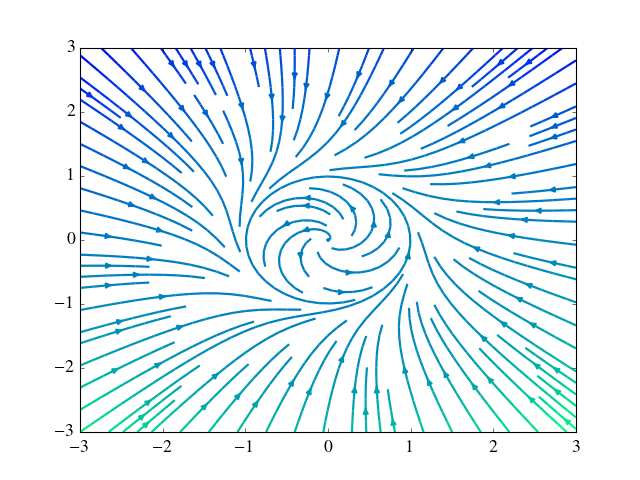
\includegraphics[scale=0.5]{problema1fig1}
\caption{Problema 1 parte 1}
\label{fig:problema1fig1}
\end{figure}


\vspace{.3cm}

Podemos ver que claramente hay un punto crítico en el origen y que coexisten 
en el espacio de fases un foco estable y uno inestable, donde obviamente debe haber
una separación entre ellos para que puedan convivir en el espacio, la cual se puede
observar claramente también.

\vspace{.3cm}

El código\footnote{La mayoría de los códigos que se utilizaron para hacer
las gráficas y figuras de esta tarea se encuentran en el repositorio 
mencionado} que finalmente hace el gráfico de la figura (\ref{fig:problema1fig1}) es el siguiente:

\begin{lstlisting}[language=Python]
Y, X = np.mgrid[-3:3:100j, -3:3:100j]
a = np.mgrid[-10:10:100j]
U = X - Y - X*(X**2+Y**2)
V = X + Y - Y*(X**2+Y**2)

plt.streamplot(X, Y, U, V,color=V,density=[1.2, 1.2], 
	      linewidth=2, cmap=plt.cm.winter)

plt.show()
\end{lstlisting}

Para la parte dos del problema nos piden que hagamos un análisis de los puntos críticos
y del comportamiento de las trayectorias en sus entornos. Para eso podemos reescribir
la ecuación diferencial de segundo orden como un sistema de ecuaciones diferenciales
lineales,


\begin{align}
 \begin{split}
  %
  \dot{x} &= y \\
  %
  \dot{y} &= - \epsilon y + x - x^3
 \end{split}
 \label{eq:ODEsystem1}
\end{align}

Haremos un análisis de estabilidad para estas ecuaciones de una forma muy conocida, utilizando
la matriz jacobiana y estudiando el comportamiento de los puntos críticos en la misma,
lo cual nos dará información sobre el comportamiento de las trayectorias en sus entornos.

\vspace{.3cm}

Para eso escribiremos (\ref{eq:ODEsystem1}) de la siguiente forma

\begin{align}
 \begin{split}
  %
  \dot{x} &= y = f(x,y)\\
  %
  \dot{y} &= - \epsilon y + x - x^3 = g(x,y)
 \end{split}
 \label{eq:ODEsystem2}
\end{align}

Para hallar los puntos críticos hacemos $0$ a $f(x,y)$ y a $g(x,y)$ en (\ref{eq:ODEsystem2})

\begin{align}
 \begin{split}
  %
  f(x,y) &= y = 0\\
  %
  g(x,y) &= -\epsilon y + x - x^3 = \epsilon y -x + x^3  = 0
  %
 \label{eq:ODEsystem3}
 \end{split}
\end{align}

Claramente vemos de (\ref{eq:ODEsystem3}) que $y=0$ será siempre parte de los puntos críticos,
y $g(x,y)$ vemos que será cero si $x=0$, $x=1$ o $x=-1$. Por lo tanto lo puntos críticos son

\begin{align}
 \begin{split}
  %
  (0,0) \\
  %
  (1,0) \\
  %
  (-1,0) 
  %
 \label{eq:puntoscriticos1}
 \end{split}
\end{align}

Para analizar el comportamiento de las trayectorias al rededor de esos puntos, primero escribimos 
el la matriz jacobiana, que se construye como


\begin{align}
J = \begin{pmatrix}
     f_x & f_y \\
     g_x & g_y
\end{pmatrix} = \begin{pmatrix}
		0 & 1 \\
		3x^2 -1 & -\epsilon
		\end{pmatrix}
\label{eq:jacobiana1}
\end{align}

Ahora para analizar el comportamiento debemos evaluar la matriz jacobiana en los puntos
críticos y utilizar los conocidos criterios para los puntos críticos. 

\vspace{.3cm}

Para el punto crítico $(0,0)$

\begin{align}
J(0,0) = \begin{pmatrix}
     0 & 1 \\
     1 & -\epsilon
\end{pmatrix}
\label{eq:jacobiana2}
\end{align}

Para encontrar los eigenvalores de (\ref{eq:jacobiana2}) usamos la ecuación

\begin{equation}
 \lambda^2 - (\text{traza J}) \lambda + \det{J} = 0
 \label{eq:calcEigenvalores}
\end{equation}

entonces para $J(0,0)$

\begin{equation}
 \lambda^2 + \epsilon \lambda - 1 = 0
\end{equation}

Esta ecuación resulta en que los eigenvalores para $J(0,0)$ son

\begin{align}
 \begin{split}
  %
  \lambda_{1,2} = - \frac{\epsilon}{2} \pm \frac{\sqrt{\epsilon^2 + 4}}{2}
  %
 \end{split}
\end{align}

Por lo que vemos que tenemos que $\lambda_1 > 0$ y que $\lambda_2 < 0$ para todo valor
de $\epsilon$, y como ambos son reales, tendremos un punto silla. En este tipo de punto
crítico tendremos un comportamiento hiperbólico en el que los ejes coordenados son 
las asíntotas, una de las coordenadas tenderá a infinito, mientras que la otra a cero.

Para los punto crítico $(\pm 1,0)$,

\begin{align}
J(1,0) = \begin{pmatrix}
     0 & 1 \\
     2 & -\epsilon
\end{pmatrix}
\label{eq:jacobiana3s}
\end{align}

Que tiene por eigenvalores utilizando la ecuación (\ref{eq:calcEigenvalores}),

\begin{align}
 \begin{split}
  %
  \lambda_{1,2} = - \frac{\epsilon}{2} \pm \frac{\sqrt{e^2-8}}{s}
  %
 \end{split}
\end{align}

Donde vemos que si $\epsilon > 0 \wedge \epsilon > 8$ tendremos dos valores negativos
reales y un nodo estable, en el cual las trayectorias se comprimen asintóticamente hacia
cero, si $\epsilon < 0 \wedge \epsilon > 8$ tendremos dos valores positivos reales y un
nodo inestable, en este caso las trayectorias se dilatan asintóticamente hacia el infinito.
En el caso que $\epsilon > 0 \wedge \epsilon < 8$ tendremos eigenvalores complejos
pero con la parte real positiva, lo que constituye un foco inestable, en el cual las trayectorias
se alejarán exponencialmente (y asintóticamente) de cero, por último cuando $\epsilon < 0 \wedge \epsilon < 8$, tenemos
de nuevo raíces complejas pero ahora con la parte real negativa, en este caso tenemos un
foco estable, en el que las trayectorias se acercan exponencialmente (y asintóticamente) a cero.

\vspace{.3cm}

Para el caso en que $\epsilon = 0$, tendremos dos centros, es decir curvas cerradas concentricas
con el origen. Entonces podemos construir los diagramas de fase y demostrar lo que hemos dicho (arriba).


\begin{figure}[h!]
 \centering
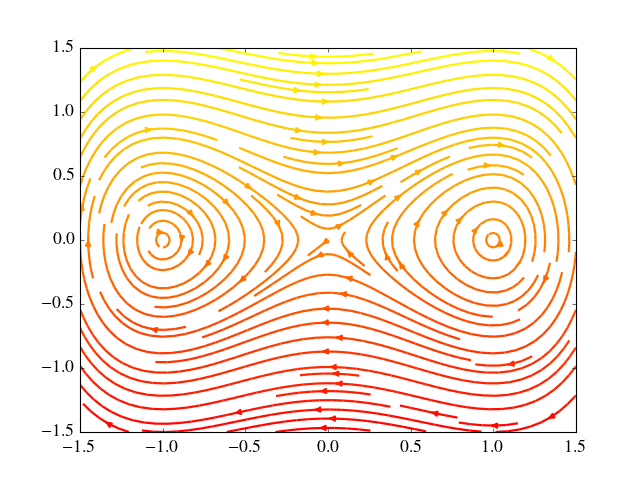
\includegraphics[scale=0.35]{problema1fig2}
\caption{Problema 1 parte 2. Centros}
\label{fig:problema1fig2}
\end{figure}

\begin{figure}[h!]
 \centering
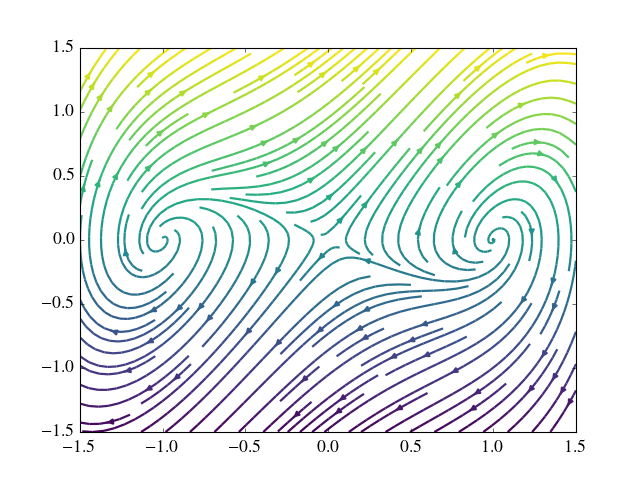
\includegraphics[scale=0.35]{problema1fig3}
\caption{Problema 1 parte 2. Focos inestables}
\label{fig:problema1fig3}
\end{figure}

\begin{figure}[h!]
 \centering
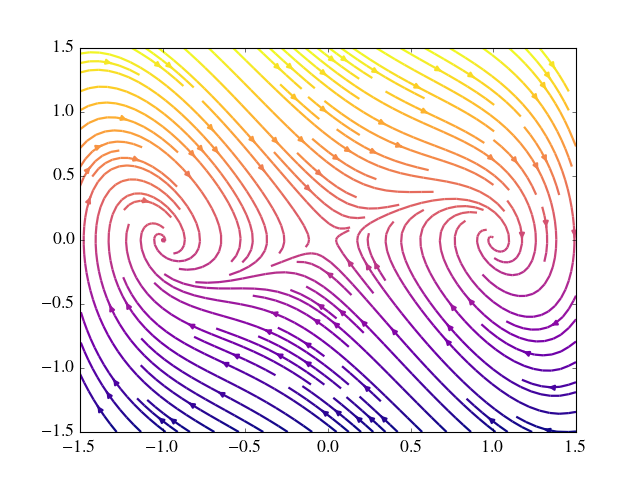
\includegraphics[scale=0.35]{problema1fig4}
\caption{Problema 1 parte 2. Focos estables}
\label{fig:problema1fig4}
\end{figure}

\begin{figure}[h!]
 \centering
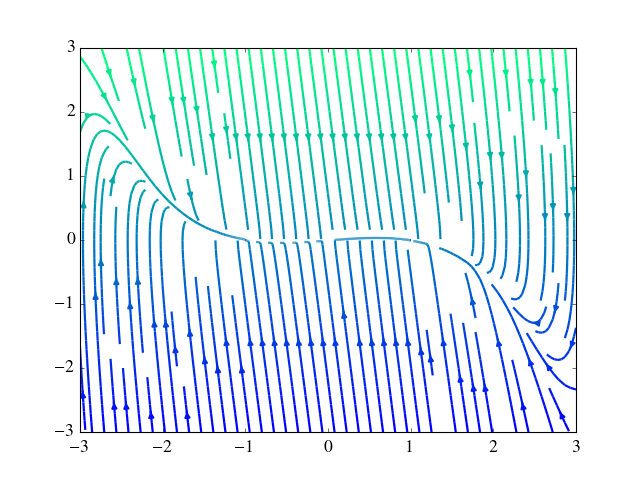
\includegraphics[scale=0.35]{problema1fig5}
\caption{Problema 1 parte 2. Nodos estables}
\label{fig:problema1fig5}
\end{figure}

\begin{figure}[h!]
 \centering
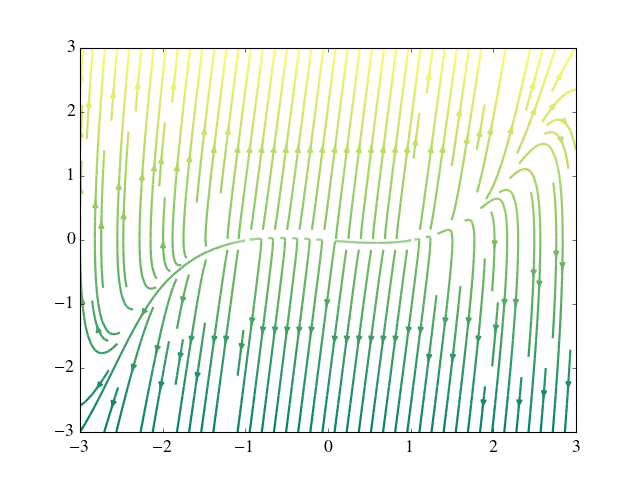
\includegraphics[scale=0.35]{problema1fig6}
\caption{Problema 1 parte 2. Nodos inestables}
\label{fig:problema1fig6}
\end{figure}

\vspace{.3cm}

\newpage
\clearpage



\section{Problema 2}

¿Podrían las funciones 

\begin{gather*}
 \begin{split}
 x(t) = at^2 + x_0, \\
 y(t) = ctx_0 + (1-t)y_0,
 \end{split}
\end{gather*}

ser la solución de una ecuación diferencial de la forma?

\begin{gather*}
 \begin{split}
 \dot{x} = f(x,y), \\
 %
 \dot{y} = g(x,y)
 \end{split}
\end{gather*}

\vspace{.3cm}

\underline{Solución:}

Si las ecuaciones dadas son soluciones de la ecuación diferencial, entonces deben
cumplir con todas las propiedades de una solución a una ecuación diferencial. Dando
un vistazo a las ecuaciones dadas, podremos demostrar que estas ecuaciones no cumplen
con todas las propiedades para ser solución a una ecuación diferencial. Principalmente
es que podemos encontrar una infinidad de valores para el cual el ``espacio de fases'' es 
multivaluado, es decir que le asigna más de un vector a un punto. Podemos ver esto de un 
modo simple, si fijamos el valor de $x_0$ como $y_0/c$, entonces obtendremos que

\begin{align}
 \begin{split}
  x(t) =  at^2 + \frac{y_0}{c} \\
  %
  y(t) = \cancel{c} t \frac{y_0}{\cancel{c}} + 1 - t y_0 = 
  \cancel{t y_0} + 1 -\cancel{t y_0} = 1
  \label{eq:ec1prob2}
 \end{split}
\end{align}

Tenemos entonces una familia de curvas que se intersectan en el punto $(a,cx_0)$. Podemos
graficar un ejemplo de estas curvas para unos valores de $a$ entre -10 y 10, y de $x_0$, igual
lo cual verifica nuestra proposición. Debido que para este valor de $x_0$, las curvas tienen
este comportamiento, es una condición suficiente para decir que estas ecuaciones no pueden
ser solución de una ecuación diferencial de la forma planteada.

\begin{figure}[h!]
 \centering
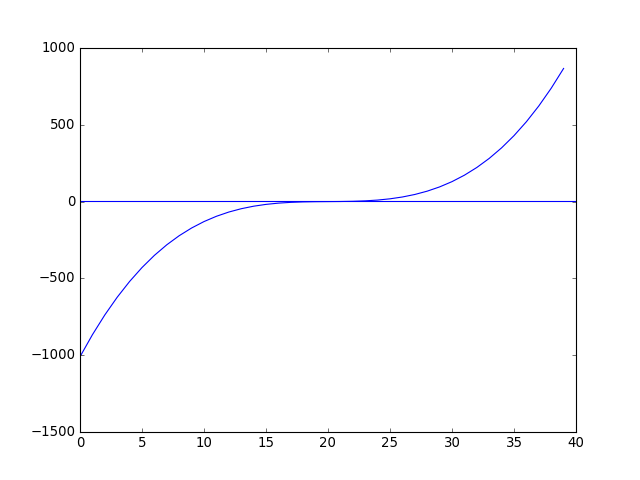
\includegraphics[scale=0.3]{problema2fig1}
\caption{Problema 2.}
\label{fig:problema2fig1}
\end{figure}


% \begin{figure}[h]
%  \centering
%     \subfloat{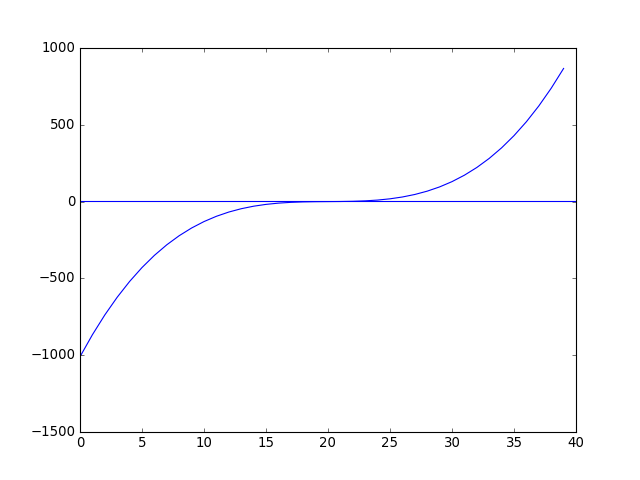
\includegraphics[scale=0.2]{problema2fig1} }%
%     \qquad
%     \subfloat{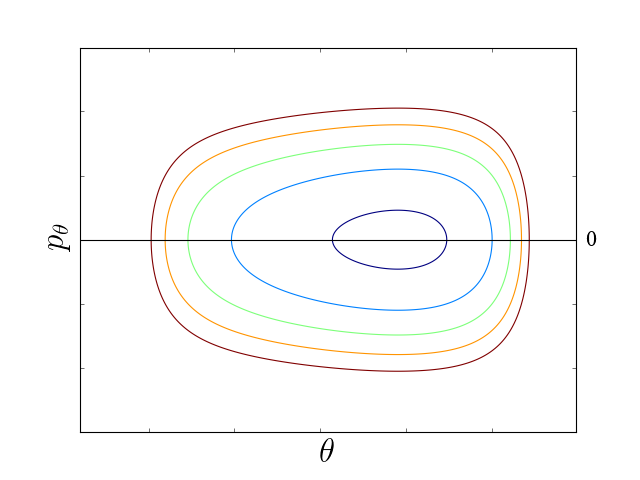
\includegraphics[scale=0.2]{problema2fig2} }%
%     \caption{Problema 2}%
%     \label{fig:example}%
% \label{fig:problema2fig1}
% \end{figure}

\vspace{.3cm}

\newpage

3.- Haga una clasificación de los puntos críticos regulares en un espacio de fase 
de tres dimensiones y trace un diagrama de fase para cada uno de ellos.

\vspace{.3cm}

\underline{Solución:}\vspace{.3cm}

En este caso la ecuación característica será cúbica real. Una ecuación cúbica real puede
tener tres raíces reales o una real y dos complejas, donde las complejas son complejas conjugadas.
Son posibles entonces varios casos, dependido del lugar de las raíces $\lambda_1, \lambda_2, \lambda_3$
en el plano de la variable compleja $\lambda$.

Para la clasificación seguiremos la de V.I Arnold en \cite{arnold}. En la cual debemos
fijarnos en el orden y signo de partes reales. Existen 10 casos ``robustos'', y una 
serie de casos ``degenerados'' cuando la parte real de una de las raíces es cero
o igual a la parte real de una raíz que no es su complejo conjugado, para la 
solución de este problema solo nos enfocaremos en estudiar los robustos. 

\vspace{.3cm}

En la figura (\ref{fig:problema3fig1}) podemos ver una representación pictórica de los
10 casos posibles que consideramos. 

\begin{figure}[h!]
 \centering
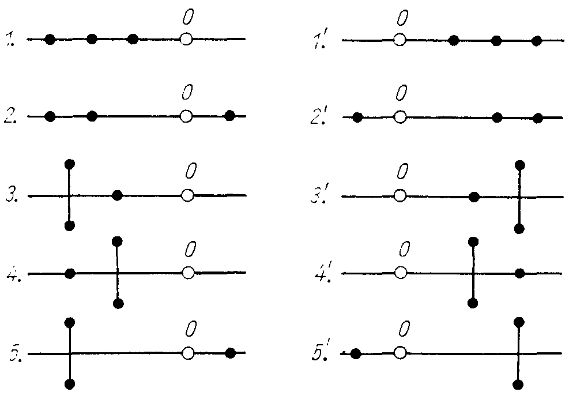
\includegraphics[scale=0.3]{problema3fig1}
\caption{Los eigenvalores de un operador real $A: \mathbb{R}^3 \rightarrow \mathbb{R}^3$}
\label{fig:problema3fig1}
\end{figure}


\textbf{Caso 1}. $\lambda_1 < \lambda_2 < \lambda_3 < 0$: El espacio de fase consiste en contracciones asintóticas
a lo largo de las tres direcciones.

\begin{figure}[H]
 \centering
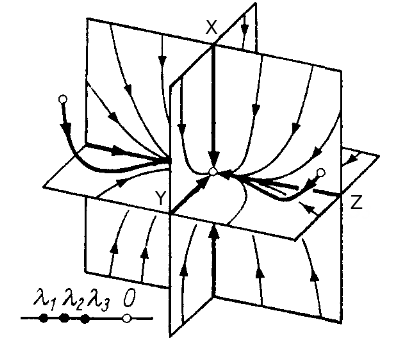
\includegraphics[scale=0.35]{problema3fig2}
\caption{Caso 1. $\lambda_1 < \lambda_2 < \lambda_3 < 0$}
\label{fig:problema3fig2}
\end{figure}
\vspace{.3cm}

\newpage

\textbf{Caso 2}. $\lambda_1 < \lambda_2 < 0 \lambda_3$: El espacio de fase consiste en contracciones asintóticas
en dos direcciones y dilatación asintótica a lo largo del tercero.

\begin{figure}[H]
 \centering
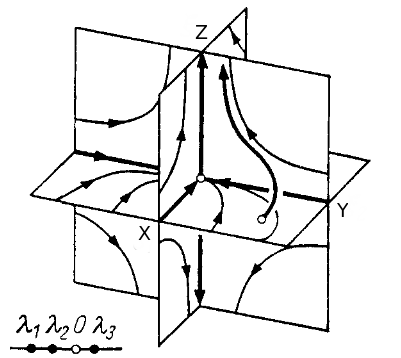
\includegraphics[scale=0.35]{problema3fig3}
\caption{Caso 2. $\lambda_1 < \lambda_2 < 0 \lambda_3$}
\label{fig:problema3fig3}
\end{figure}
\vspace{.3cm}

\textbf{Caso 3}. Re $\lambda_{1,2} < \lambda_3 < 0$ : El espacio de fase consiste en en una contracción asintótica
en la dirección de $Z$, y una rotación con una contracción asintótica más rápida en el plano
$(X,Y)$.

\begin{figure}[H]
 \centering
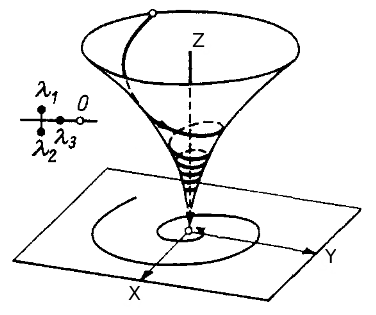
\includegraphics[scale=0.35]{problema3fig4}
\caption{Caso 3. Re $\lambda_{1,2} < \lambda_3 < 0$}
\label{fig:problema3fig4}
\end{figure}
\vspace{.3cm}

\textbf{Caso 4}. $\lambda_3 <$ Re $\lambda_{1,2} < 0$ : El espacio de fase consiste en en una contracción asintótica
en la dirección de $Z$, y una rotación con una contracción asintótica menos rápida en el plano
$(X,Y)$.

\begin{figure}[H]
 \centering
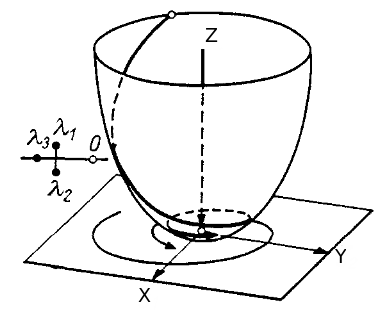
\includegraphics[scale=0.35]{problema3fig5}
\caption{Caso 4. $\lambda_3 <$ Re $\lambda_{1,2} < 0$}
\label{fig:problema3fig5}
\end{figure}
\vspace{.3cm}

\textbf{Caso 5}. Re $\lambda_{1,2} < 0 < \lambda_3$: El espacio de fase consiste en una dilatación asintótica
en la dirección de $Z$, y rotación con contracción asintótica en el plano $(X,Y)$

\begin{figure}[H]
 \centering
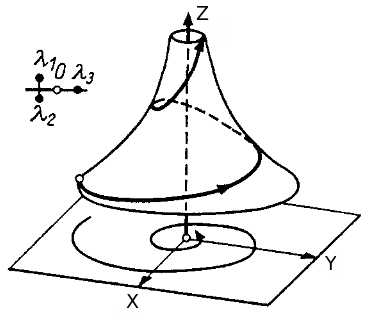
\includegraphics[scale=0.35]{problema3fig6}
\caption{Caso 5. Re $\lambda_{1,2} < 0 < \lambda_3$}
\label{fig:problema3fig6}
\end{figure}
\vspace{.3cm}

\textbf{Caso 6}. $\lambda_1 > \lambda_2 > \lambda_3 > 0$: El espacio de fase consiste en dilataciones asintóticas
a lo largo de las tres direcciones.

\begin{figure}[h]
 \centering
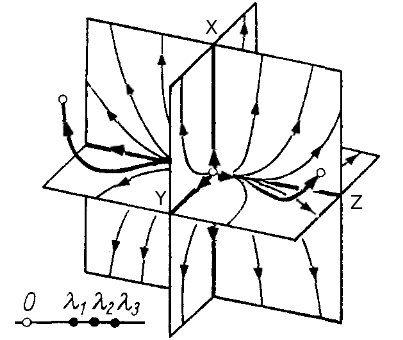
\includegraphics[scale=0.35]{problema3fig7}
\caption{Caso 6. $\lambda_1 > \lambda_2 > \lambda_3 > 0$}
\label{fig:problema3fig7}
\end{figure}
\vspace{.3cm}

\textbf{Caso 7}. $\lambda_3 < 0 < \lambda_1 < \lambda_2$: El espacio de fase consiste en dilataciones asintóticas
en dos direcciones y contracción asintótica en la tercera.

\begin{figure}[h!]
 \centering
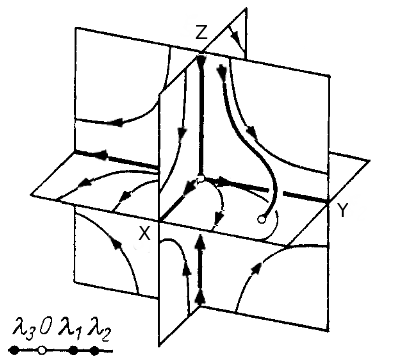
\includegraphics[scale=0.35]{problema3fig8}
\caption{Caso 7. $\lambda_3 < 0 < \lambda_1 < \lambda_2$}
\label{fig:problema3fig8}
\end{figure}
\vspace{.3cm}

\textbf{Caso 8}. $0 > \lambda_3 > $ Re $\lambda_{1,2}$: El espacio de fase consiste en una dilatación asintótica en 
la dirección de $Z$ y rotación con una dilatación más rápida en el plano $(X,Y)$.

\begin{figure}[h!]
 \centering
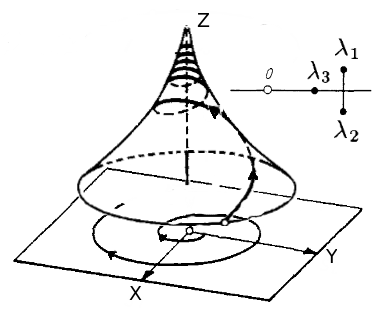
\includegraphics[scale=0.35]{problema3fig9}
\caption{Caso 8. $0 > \lambda_3 > $ Re $\lambda_{1,2}$}
\label{fig:problema3fig9}
\end{figure}
\vspace{.3cm}

\textbf{Caso 9}. $0 > $ Re $\lambda_{1,2} > \lambda_3$. El espacio de fases consiste en una dilatación asintótica
en la dirección de $Z$, y rotación con una dilatación asintótica menos rápida en el plano $(X,Y)$.

\begin{figure}[h!]
 \centering
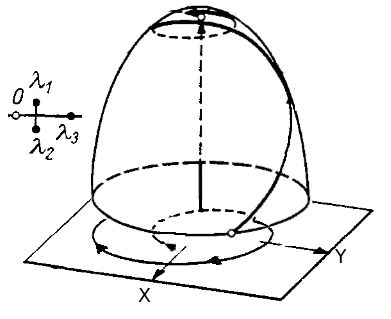
\includegraphics[scale=0.35]{problema3fig10}
\caption{Caso 9. $0 > $ Re $\lambda_{1,2} > \lambda_3$}
\label{fig:problema3fig10}
\end{figure}
\vspace{.3cm}

\textbf{Caso 10}. $\lambda_3 > 0 > $ Re $\lambda_{1,2}$. El espacio de fases consisten en una contracción asintótica
en la dirección de $Z$, y una dilatación asintótica en el plano $(X,Y)$.

\begin{figure}[h!]
 \centering
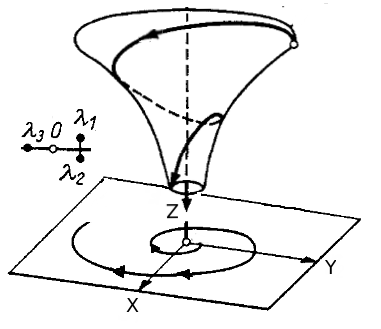
\includegraphics[scale=0.35]{problema3fig11}
\caption{Caso 10. $\lambda_3 > 0 > $ Re $\lambda_{1,2}$}
\label{fig:problema3fig11}
\end{figure}
\vspace{.3cm}

\newpage

4.- Se han encontrado cuatro puntos críticos de una ecuación diferencial en la esfera
de dos dimensiones ($R^2$ cerrado al incluir el punto al infinito). Uno es un foco
estable y los otros tres son puntos silla. ¿Será posible que la ecuación no tenga
más puntos críticos? Explique su respuesta.


\vspace{.3cm}

\underline{Solución:}

\vspace{.3cm}

5.- Dé una demostración formal de la equivalencia matemática entre una ecuación
diferencial y un flujo.

\vspace{.3cm}

\underline{Solución:}\vspace{.3cm}

Para poder demostrar la equivalencia matemática entre una ecuación diferencial y un flujo,
primero hay que demostrar la equivalencia entre una ecuación diferencial y un campo vectorial.

\vspace{.3cm}

Asumamos que en cada punto de una cierta región del plano, se ha escogido una línea
recta que pasa por este punto. En este caso diremos en que ha sido definido un campo
direccional en la región. Se dice que un campo direccional es continuo si las lineas
en el campo dependen continuamente del punto de adjunción. Una línea, que en cada uno
de sus puntos, es tangente a un campo vectorial es llamada una línea integral del
campo direccional.

\vspace{.3cm}

El problema geométrico de encontrar curvas integrales es escrito analíticamente como el
problema de encontrar soluciones a una ecuación diferencial. Una condición necesaria 
y suficiente para que el gráfico de una función $\phi$ sea una curva integral 
es que se cumpla la siguiente relación para todo $t$ en un intervalo dado:


\vspace{.3cm}


\begin{thebibliography}{10}
 \bibitem{arnold}
 V.I. Arnold, \emph{Ordinary Differential Equations}, Springer-Verlang,
 3ra edición, 1992.
\end{thebibliography}



\end{document}
